\scanpage{172}
\margin{\uline{à vérifier !}}
\margin{\unsure{Généraliser} : aux faisceaux d'anneaux ``\unsure{plus généraux}''.}
\uline{Théorème} Soit $X$ de type \inserted{loc} fini sur le corps $k$, $\dim X\leq n$, $A=\mathbb{Z}/N\mathbb{Z}$, $N$ premier à car. $k$, \deleted{\unsure{Alors}} \inserted{$F$} et $C$ deux $A$-\deleted{\unsure{ét.}}Modules. Supposons que $F$ soit plat $=$ $C$ : fibres injectives ($=$ plates, dans le cas particulier envisagé !). Alors

(i) Si $F$ constructible, alors $\operatorname{Ext}^i(F,\unsure{G|C})=0$ pour $i>2n$.

(ii) Si $k$ est séparablement clos, alors \deleted{\unsure{pour tout}}
\[
\begin{aligned}
\unsure{\mathcal{E}xt^i|\operatorname{Ext}^i}(\deleted{\unsure{A}}\inserted{F},C)&=0&\text{pour }i&>2n\\
\operatorname{Ext}^i(F,C)&=0&\text{pour }i&>2n.
\end{aligned}
\]

\uline{Dém.} (i) se ramène par passage à la limite à (ii). Dans (ii), on peut supposer $k$ sép. clos, et \deleted{un argument général} il suffit de prouver le \uline{premier} alinéa. \inserted{supposer d'abord $C$ : fibres injectives.} Un argument général nous ramène à \deleted{\unsure{le}} vérifier \inserted{la formule} lorsque $F$ est \unsure{quotient} d'un \unsure{produit|générateur} de la forme $i_!(A_{X'})$, où $X'$ affine et $X'\unsure{-|\longrightarrow}X$ étale, \unsure{au} dessus d'un ouvert affine \inserted{$U$} de $X$. Car on se ramène au cas où $X=U$ est aussi affine [car on peut remplacer $X$ par $U$, $C$ par $C|U$]
\margin{\figure{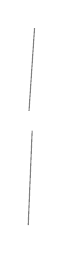
\begin{tikzpicture}[x=1cm,y=1cm]\draw[gray] (0,0)--(0.05,1.2);\draw[gray] (0.01,1.45)--(0.08,2.5);\end{tikzpicture}}}
\margin{171}
